% This file can be used to compile the adventure into a stand alone PDF without the sourcebook
\documentclass{book}


\usepackage{../../static/templates/fate_latex_template/fate_solarpunk_de}
\usepackage{montserrat}
\usepackage{ebgaramond}
\usepackage{hyperref}
\usepackage{graphicx}

%%%%%% Fixing overful hboxes
%% https://tex.stackexchange.com/questions/35/what-does-overfull-hbox-mean-why-is-there-a-black-mark-at-the-end-of-a-line
\usepackage{hyphenat}
%% \hyp{} can mark where words can break
%% Make it simpler:
%% https://tex.stackexchange.com/questions/488008/how-to-create-an-alternative-to-shortcut-or-hyp
\usepackage[german]{babel}

\usepackage[pages=some]{background}
\backgroundsetup{
scale=1,
angle=0,
opacity=1,
firstpage=true,
contents={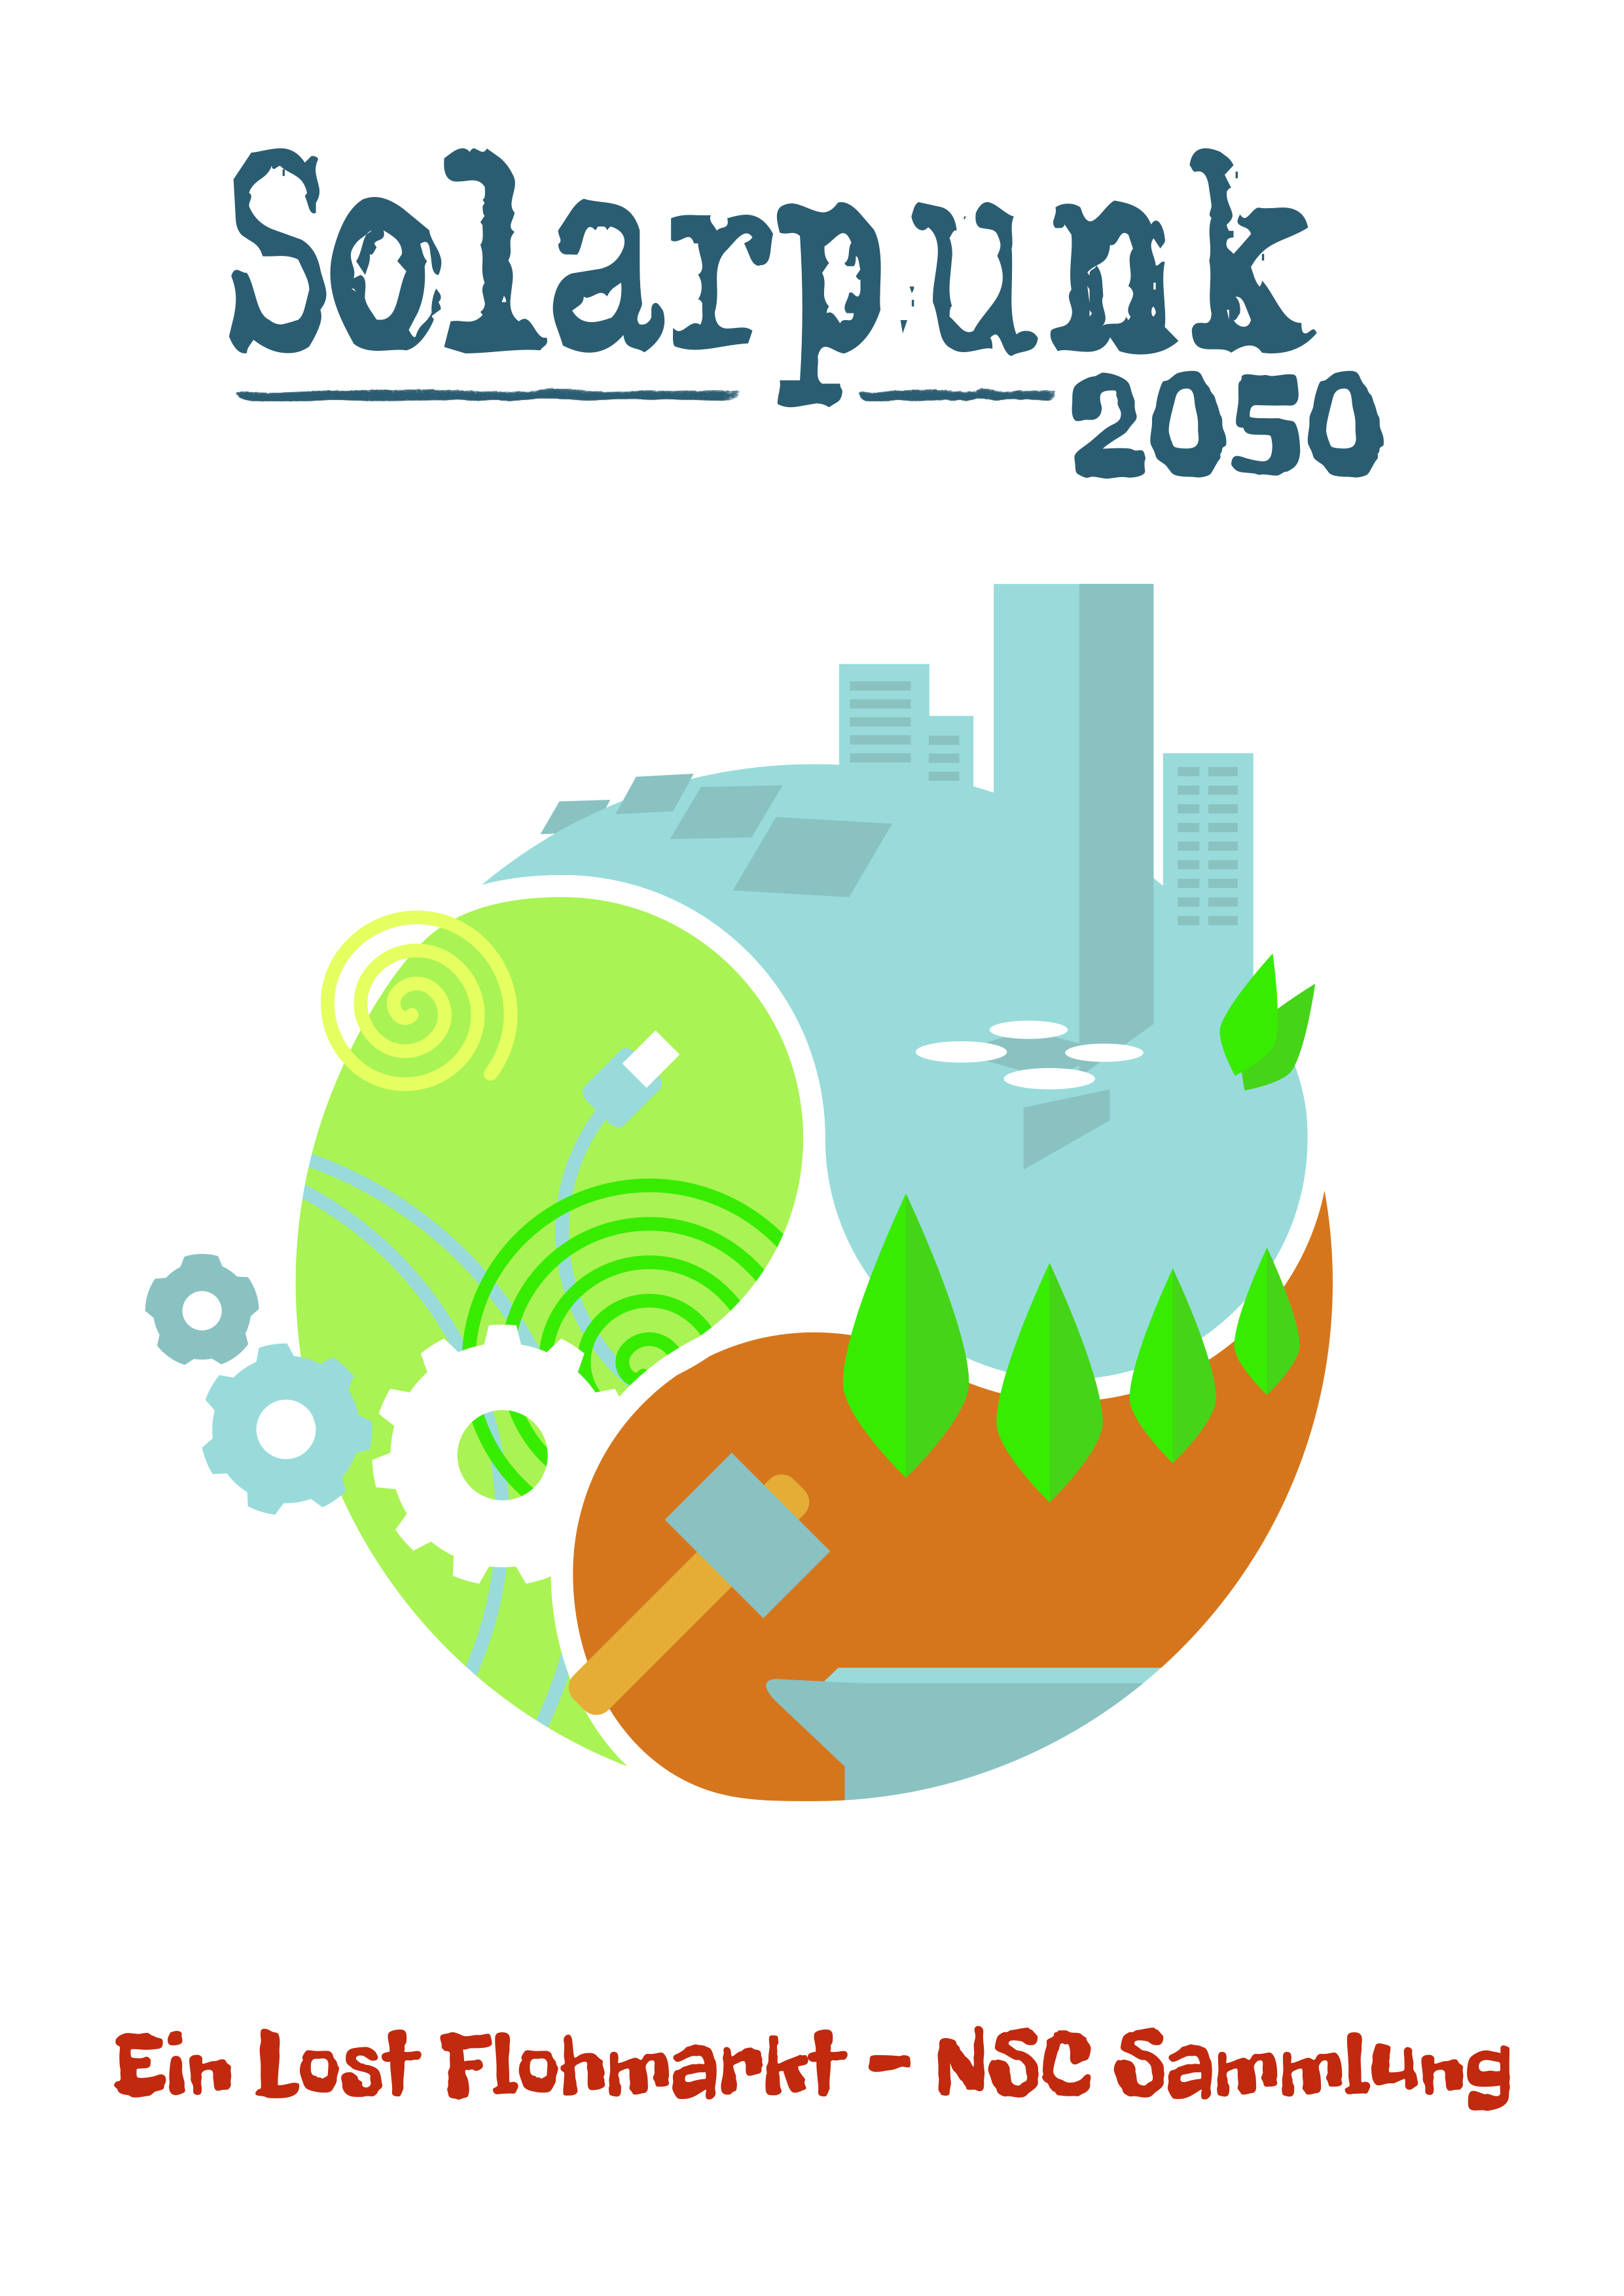
\includegraphics[width=\paperwidth,height=\paperheight]{../sourcebook/static/Solarpunk-Lost-Flohmarkt-de.png}}
}

\useshorthands{~}
\defineshorthand{~-}{\hyp{}}




%... other code

% \section{Hello World}
% \label{sec:hello}



% For creating example text
% \usepackage{lipsum}

\title{Fate Solarpunk 2050 - Der Lost Flohmarkt}
\author{Thorsten Sick}

\pagenumbering{arabic}
\begin{document}

%
% Book front page
%
\mbox{}
\thispagestyle{empty}
\BgThispage

\newpage
\begin{center}
\textbf{Text and idea}
\newline
Thorsten Sick
\newline
\textbf{Visuals}
\newline
Mullana ( https://mullana.de/ )
\newline
\textbf{Test players}
\newline
Michael, Ingrid, Susanne Peschl
\newline
\end{center}
\newpage

% Hyphenation database:
\hyphenation{meal-worm Mc-Gyver fa-mous be-cause}
%

\chapter{Einleitung}

Solarpunk ist ein utopisches Science Fiction Genre. \textbf{Solarpunk 2050} ist ein Setting in dem das Ziel der Utopie fast erreicht ist. Aber noch ist die Solarpunk Revolution im Gange. Drei Gruppen haben großartige Visionen für eine bessere Zukunft. Doch diese unterscheiden sich.

Die Lost Vision umfasst ein naturnahes Leben basierend auf der Weisheit der Vorfahren. Sie scheuen Technologie, die Mikrokontroller enthälten. Sind aber sehr kompetent im Gebrauch älterer Technologien.

Die Pioneer Vision ist entgegengesetzt. Die Individualisten finden sich zusammen um ständig an neuen Technologien und am Fortschritt zu experimentieren - großartige Durchbrüche werden aber teils teuer erkauft durch Unfälle. Eine ständige Party der Wissenschaft und der neuen Erkenntnisse findet dort statt.

Die Norm Gesellschaft basiert auf älteren Erkenntnissen der Pioneers. In der durch die Hive AI koordinierten Gesellschaft ist alles hochautomatisiert und vernetzt. Norms sind niemals alleine sondern ständig per Hive Controller mit allen in der Gemeinde und der AI verbunden. Der Basisbedarf (Essen, Wohnen, Transport) ist kostenlos, da es aus erneuerbaren Materialien und vollautomatisch hergestellt wird. Darum können sich Norms auf die Schaffung neuer Kultur und Arbeit-als-Hobby fokussieren.

\textbf[In diesem Abenteuerbaustein geht es um einen Lost Flohmarkt und einige zentrale damit verbundenen Menschen. Denn auf diesen Flohmärkten treffen sich Losts aus verschiedenen Gruppen. Friedlich.
Es gib Erfahrungsaustausch, Tauschhandel, Handwerker und Kultur. Und das eine oder andere Abenteuer kann hier beginnen.}

Das hier kann als Abenteuer verwendet werden (mit genug Drama für eine Telenovella), als Plot hooks, als Zwischenspiel, als Sammlung von NSCs oder doch als fertige Spielercharaktere.

Das Setting ist für die \href{https://fate-srd.com/fate-condensed}{Fate Condensed} Regeln geschrieben, kann aber einfach adaptiert werden.

% Ziele: Story hooks
% Mehr Drama als eine Telenovella
% Man muss zig Abenteuer aus der Konstellation ziehen können
% Die Meisten Charaktere sind ü 60 und haben viel erlebt. Das aufzählen.

\chapter{Der Lost Flohmarkt}

Es gibt mehrere Lost Flohmärkte. Dieser hier ist ein mobiler, durch die Lande ziehender Flohmarkt und Treffpunkt verschiedener Lost Gruppen. Doch auch einige Norms und Pioneers werden von diesem angezogen und of verwirrt zurück gelassen.

Für die Lost ist die Funk Nachricht, dass bald ein Flohmarkt in ihrer Nähe stattfinden wird ein wichtiges Ereignis. Doch diesen zu organisieren bedarf einiges an Aufwand und spezieller Menschen.

Am wertvollsten sind die Artefakte aus der alten Welt, die die Lost bei Expeditionen geborgen haben. Die Artefakte der Lemminge. Insbesondere die Lost sind auf alte Technologie angewiesen, um ihre Fahrzeuge und Gebäude zu reparieren.

Lost handeln übrigens im Tauschhandel, Norms bezahlen mit digitalem Geld und bei Pioneers finden viele Transaktionen eher über Ruf und Ruhm der Personen statt. Auf einem Lost Flohmarkt sind also gerade für nicht-Lost Kulturschocks und chaotische Ketten an Tauschhandel vorprogrammiert.

\section{Der erstrebte Flohmarkt}

Wenn alle Probleme beseitig sind, ist der Flohmarkt eine binte Mischung aus Essensdüften, unplugged Musik, Handel und Gefeilsche, Theater, dem Lärm von Schmieden und Tieren. Allgemein ein großes low tech Festival an dem sich verschiedene sonst verfeindete Gruppen treffen.
Freundschaften werden geschlossen. Pläne geschmiedet und Waren, Geschichten und Gerüchte ausgetauscht.

Nachte beleuchtet von Fackeln und verteilten Lagerfeuern. Gespräche, Gesang und Geschichten bis spät in die Nacht. Es wird getrunken, geraucht und gegessen.

Ca 2 Wochen lange lebt der Ort mit 500 Leuten vor Ort (wobei dauernd an und Abreisen stattfinden).

Wie immer sind in den Abenteuern viele 'Grüne Inseln der Ruhe' einzubauen. Wo nach irgendwelchen Beinahekatastrophen einfach alles schön ist. Das stärkt das Solarpunk Feeling im Spiel. Der Flohmarkt kann sehr viele schöne Facetten für die SC bieten.

Großartige Dinge, die passieren können:

\subsection{Zufallsereignisse}

\begin{enumerate}
    \item Jacob will sein geheimes Badewannen-Gin Rezept nicht mit ins Grab nehmen. Den ersten drei Personen, die ihm besondere Spirituosen bringen wird er es beibringen.
    \item Nachts gibt es eine spontante Feuer Jonglage show
    \item Jemand macht ein Quiz 'Die 1980er Jahre'. zu gewinnen gibt es eine Flasche von Jabobs Badewannen-Gin
    \item Zwei Personen haben sich verlobt. Um das zu feiern kommt eine ganze Sau auf den Grill - das duftet den ganzen Tag über den Flohmarkt. Norms und Pioneers könnten verwirrt reagieren.
    \item Ein Wettstreit. Zwei Gruppen wollen sich bei Shakespear Darbietungen überbieten. Doch noch fehlen einige passende Personen bei der Besetzung
    \item Erwachsene und Kinder ab 14 können beider Spontant aufgebauten Schießanlage mit Halbautomatischen Waffen üben. Norms sind sicher irritiert.
\end{enumerate}


\chapter{Die Aufgabe}

Das Team des Flohmarkts reist durch die Lande, kündigt einen Flohmarkt an, organisiert einen Platz und beginnt diesen herzurichten für um die 500 Personen. Viele der dazukommenden Lost werden zwar selbst beitragen (eigene Essens Stände, Werkstätten).
Doch das Team stellt die Basisinfrastruktur zur Verfügung und versucht verfeindete Gruppen zusammen zu bringen. Denn das ist der sinn des Flohmarkts (neben Tauschhandel, Wissensaustausch, Unterhaltung).

\section{Die Probleme}

Beim Aufbau des Lost Flohmarktes kommt es natürlich zu einer Reihe von Problemen. Diese müssen von den NSCs, den Protagonisten und evtl. den neu hinzugekommenen Gruppen gelöst werden. Sollte die Situation mit externen Charakteren als Protagonisten gespielt werden, wäre es eine coole Herausforderung, die Flohmarkt-NSCs die großen Herausforderungen stemmen zu lassen, und den PC Protagonisten die Rolle des Steine-aus-dem-Weg räumens und als Katalysator zukommen zu lassen. Die Listen haben jeweils 6 Einträge. Falls die Spielleiterin das auswürfeln will. Ereignisse kommen immer in der schlimmstmöglichen Kombination zum ungeschicktesten Zeitpunkt.

\subsection{Zufallsereignisse beim Aufbau}

\begin{enumerate}
\item Eine Gruppe kommt zu spät (Was ist passiert ?)
\item Eine Gruppe kommt zu früh (Warum ?)
\item Das Feld auf dem der Flohmarkt stattfinden soll ist nach Starkregen ein See. Mit Brennesseln und Gestrüpp. Der muss zuerst mit schwerem Gerät trocken gelegt werden.
\item Beim Aufbau wird eine verschüttete Lemming Ruine gefunden. Die Jones-es wollen diese durchsuchen. Das kann zu einem Dungeon Crawl führen.
\item Der Aufbau wird verlangsamt, weil die Küche die Leute mit lecker Essen vom arbeiten abhält
\item Neugierige Kinder aus dem nahen Pioneer Labor kommen mit ihren Exoskeletten zu besuch - Die Lost reagieren zwischen ängstlich (wegen der Technik) und behütend
\end{enumerate}

\chapter{Die Personen}

\section{Tier Experte: Jonas Ohnesorg}

Organisiert die Unterbringung der Tiere (von Hasen bis zu Rindern). Sorgt für die Gesundheit der verkauften Tiere und hilft bei der Futterversorgung. Ist aber eigentlich Tiertrainer für Raubvögel. Diese reissen aber manchmal Hasen - auch solche in den Freigehegen der Farmer.

\newpage
\begin{npcBox}[title=Jonas Ohnesorg]

    \begin{aspects}
    \item \aspect[Konzept]{Liebt die Tiere mehr als sie ihn lieben}
    \item \aspect[Dilemma]{Irgendwas ermutigt andere immer, seine Tiere unsachgemäß anfassen zu wollen}
    \item \aspect[Beziehung]{Ist in Antigone verliebt}
    \item \aspect[Aspekt]{TODO}
    \end{aspects}

    \begin{skills}
    \item \nskill{Bildung}{0}
    \item \nskill{Athletik}{1}
    \item \nskill{Diebeskunst}{0}
    \item \nskill{Kontakte}{1}
    \item \nskill{Handwerk}{3}
    \item \nskill{Täuschung}{0}
    \item \nskill{Fahren}{0}
    \item \nskill{Empathie}{1}
    \item \nskill{Kämpfen}{3}
    \item \nskill{Nachforschung}{0}
    \item \nskill{Spezialwissen}{0}
    \item \nskill{Wahrnehmung}{1}
    \item \nskill{Kraft}{2}
    \item \nskill{Provozieren}{0}
    \item \nskill{Charisma}{2}
    \item \nskill{Ressourcen}{0}
    \item \nskill{Schießen}{0}
    \item \nskill{Heimlichkeit}{0}
    \item \nskill{Wille}{2}
    \item \nskill{Bushcraft}{4}
    \end{skills}

    \begin{stunts}
    \item \stunt{TODO}{Bar}
    \end{stunts}

    \begin{stressSection}
    \stressLine{\stress{1}\stress{1}\stress{1}\stress{1}\stress{1}\stress{1}}{\stress{1}\stress{1}\stress{1}\stress{1}}
    \end{stressSection}
    \begin{tabularx}{\textwidth}{ XX }
    \end{tabularx}

    \begin{consequences}
    \item \consequence{2}
    \item \consequence{4}
    \item \consequence{6}
    \end{consequences}

    \begin{npcDescription}
    TODO
    \end{npcDescription}


    \begin{equipment}
    \item TODO
    \end{equipment}
\end{npcBox}


\subsection{Zufallsereignisse mit Tieren}

\begin{enumerate}
\item Ein Tier bricht aus
\item Ein Tier ist krank - eine Seuchengefahr ? Findet jemand einen (Tier) Arzt ?
\item Trächtige Tiere bekommen ihre Jungen
\item Norms oder Pioneers sind verwirrt von den Tieren. Wollen die streicheln, behalten oder filmen - was schief geht
\item Den Tieren gehlt Futter. Jemand muss schnell richtig viel besorgen
\item Seine Raubvögel reissen anderer Leute Kleintiere
\end{enumerate}

\newpage
\section{Küche und Militärtaktik}

Name: Gustav Müller
Ordnung, Disziplin und die Saucen sind zentral !
Lieblings-doofer Spruch: 'Kein Mampf, kein Kampf'

Zwischen dem Führen einer Küche und einer Schlacht Organisation gibt es kaum Unterschiede'. Führen kleiner Einheiten. Zur Lager Verteidigung oder beim Kochen für einen Flohmarkt. https://de.wikipedia.org/wiki/K%C3%BCchenbrigade
Feldküche und Feld Taktik.

\newpage
\begin{npcBox}[title=Gustav Müller]

    \begin{aspects}
    \item \aspect[Konzept]{Perfekt organisierter Küchengeneral}
    \item \aspect[Dilemma]{Hart zu sich selbst - bis zum umfallen}
    \item \aspect[Beziehung]{Er hat keine engeren Beziehungen zu Menschen}
    \item \aspect[Aspekt]{TODO}
    \end{aspects}

    \begin{skills}
    \item \nskill{Bildung}{0}
    \item \nskill{Athletik}{1}
    \item \nskill{Diebeskunst}{0}
    \item \nskill{Kontakte}{0}
    \item \nskill{Handwerk - Kochen}{3}
    \item \nskill{Täuschung}{0}
    \item \nskill{Fahren}{1}
    \item \nskill{Empathie}{0}
    \item \nskill{Kämpfen}{1}
    \item \nskill{Nachforschung}{0}
    \item \nskill{Spezialwissen}{2}
    \item \nskill{Wahrnehmung}{1}
    \item \nskill{Kraft}{2}
    \item \nskill{Provozieren}{2}
    \item \nskill{Charisma}{0}
    \item \nskill{Ressourcen}{0}
    \item \nskill{Schießen}{3}
    \item \nskill{Heimlichkeit}{0}
    \item \nskill{Wille}{4}
    \end{skills}

    \begin{stunts}
    \item \stunt{TODO}{Bar}
    \end{stunts}

    \begin{stressSection}
    \stressLine{\stress{1}\stress{1}\stress{1}\stress{1}\stress{1}\stress{1}}{\stress{1}\stress{1}\stress{1}\stress{1}}
    \end{stressSection}
    \begin{tabularx}{\textwidth}{ XX }
    \end{tabularx}

    \begin{consequences}
    \item \consequence{2}
    \item \consequence{4}
    \item \consequence{6}
    \end{consequences}

    \begin{npcDescription}
    TODO
    \end{npcDescription}


    \begin{equipment}
    \item TODO
    \end{equipment}
\end{npcBox}


\subsection{Zufallsereignisse}

\begin{enumerate}
\item Auf einem LKW ist ein Kräutergarten angelegt. Der steht aber nicht bei den Küchenzelten - weil den jemand vergessen hat. Der muss jetzt irgendwie durch den halb aufgebauten Flohmarkt gefahren werden.
\item Man muss aus einem alten Diesel Motor und Getriebe schnell ein riesen Rührwerk improvisieren
\item Eine riesen Tafel wird an einem Tag quer durch den Flohmarkt aufgebaut und alle erhalten ein Festmahl - wenn es denn klappt
\item Gustav überlässt die Küche für ein paar Stunden einem Vertrauten. Er muss sich um Kampftaktik Übungen im nahen Wald kümmern
\item Er wird gefragt, ob er Schießtraining für Kinder und Erwachsene anieten kann. Kann er - wenn er Hilfe bei der Küche und der noch zu bauenden Schießanlage bekommt.
\item Leute werden unsaft aus der Küche geworfen
\end{enumerate}

\newpage

\section{Funk: Antigone Freitag}

Sie kennt jeden, kann viele Sprachen. Will Sammelfiguren komplett bekommen: Fragt bei seinen Funk Kontakten rum und kann evtl. eine Bergungstrupp losschicken wollen. Selbst sitzt sie im Rollstuhl. Per Funkgerät kommt aber die gesamte Welt zu ihr.

\newpage
\begin{npcBox}[title=Antigone]

    \begin{aspects}
    \item \aspect[Konzept]{Funkerin und Soziale Enzyklopädie}
    \item \aspect[Dilemma]{Kennt fast jeden eng - hat aber oft keine Ahnung wie sie aussehen}
    \item \aspect[Beziehung]{Dadurch, dass sie jeden sehr gut kennt, hat sie niemanden speziellen}
    \item \aspect[Aspekt]{TODO}
    \end{aspects}

    \begin{skills}
    \item \nskill{Bildung}{3}
    \item \nskill{Athletik}{1}
    \item \nskill{Diebeskunst}{0}
    \item \nskill{Kontakte}{3}
    \item \nskill{Handwerk - Funktechnik}{2}
    \item \nskill{Täuschung}{0}
    \item \nskill{Fahren}{0}
    \item \nskill{Empathie}{2}
    \item \nskill{Kämpfen}{0}
    \item \nskill{Nachforschung}{1}
    \item \nskill{Spezialwissen}{1}
    \item \nskill{Wahrnehmung}{2}
    \item \nskill{Kraft}{0}
    \item \nskill{Provozieren}{0}
    \item \nskill{Charisma}{4}
    \item \nskill{Ressourcen}{0}
    \item \nskill{Schießen}{0}
    \item \nskill{Heimlichkeit}{0}
    \item \nskill{Wille}{1}
    \end{skills}

    \begin{stunts}
    \item \stunt{TODO}{Bar}
    \end{stunts}

    \begin{stressSection}
    \stressLine{\stress{1}\stress{1}\stress{1}\stress{1}\stress{1}\stress{1}}{\stress{1}\stress{1}\stress{1}\stress{1}}
    \end{stressSection}
    \begin{tabularx}{\textwidth}{ XX }
    \end{tabularx}

    \begin{consequences}
    \item \consequence{2}
    \item \consequence{4}
    \item \consequence{6}
    \end{consequences}

    \begin{npcDescription}
    TODO
    \end{npcDescription}


    \begin{equipment}
    \item TODO
    \end{equipment}
\end{npcBox}

\subsection{Zufallsereignisse}

\begin{enumerate}
\item Sie hat jemanden per Funk gefunden, der Sammelfiguren hat. Und die Person ist auf dem Flohmarkt. Da kein Funkkontakt besteht, müssen die Protagonisten die Person per Beschreibung finden
\item Eine anreisende Truppe ist in Gefahr und die PC müssen sie her leiten
\item Funkrepeater müssen gebaut und an Gruppen verteilt werden, die bald abreisen
\item Das Funkgerät fällt aus. Schnell wird ein Verstärker und eine Elektronikerin benötigt
\item Sie will den Flohmarkt auch mal durchreisen. Nur ist der Rollstuhl unpraktisch im Schlamm. Sie braucht Hilfe. Bei der Reise wird sie viele der Leute zum ersten mal sehen, mit denen sie sonst nur redet.
\item Sie will ein Flohmarkt-Radioprogramm senden. Empfänger müssen verteilt werden und Inhalt erstellt.
\end{enumerate}

\newpage

\section{Gaia Priester}

Laura, Gaianistin. Sie ist eine unerfahrene Priesterin, in einer sich selbst gerade gründenden Religion. Da sie abgeschieden ist, ist sie für jeden spirituellen Input (Bücher, Gespräche) sehr dankbar. Oft versucht sie auch, anderen Gaia zu erklären - stolpert dabei aber schnell, sobald es komplexer wird.

\newpage
\begin{npcBox}[title=Laura, Gaianistin]

    \begin{aspects}
    \item \aspect[Konzept]{Beginnende Gaianistin}
    \item \aspect[Dilemma]{Die Schuhe sind zu groß}
    \item \aspect[Beziehung]{Sie hat sich frisch der Flohmarkt Gruppe angeschlossen und kennt noch niemanden}
    \item \aspect[Aspekt]{Frisch den weg gefunden, hoch begeistert und noch stoplernd}
    \end{aspects}

    \begin{skills}
    \item \nskill{Bildung}{3}
    \item \nskill{Athletik}{1}
    \item \nskill{Diebeskunst}{0}
    \item \nskill{Kontakte}{1}
    \item \nskill{Handwerk}{0}
    \item \nskill{Täuschung}{0}
    \item \nskill{Fahren}{0}
    \item \nskill{Empathie}{3}
    \item \nskill{Kämpfen}{0}
    \item \nskill{Nachforschung}{2}
    \item \nskill{Spezialwissen}{2}
    \item \nskill{Wahrnehmung}{1}
    \item \nskill{Kraft}{0}
    \item \nskill{Provozieren}{0}
    \item \nskill{Charisma}{4}
    \item \nskill{Ressourcen}{1}
    \item \nskill{Schießen}{0}
    \item \nskill{Heimlichkeit}{0}
    \item \nskill{Wille}{2}
    \end{skills}

    \begin{stunts}
    \item \stunt{TODO}{Bar}
    \end{stunts}

    \begin{stressSection}
    \stressLine{\stress{1}\stress{1}\stress{1}\stress{1}\stress{1}\stress{1}}{\stress{1}\stress{1}\stress{1}\stress{1}}
    \end{stressSection}
    \begin{tabularx}{\textwidth}{ XX }
    \end{tabularx}

    \begin{consequences}
    \item \consequence{2}
    \item \consequence{4}
    \item \consequence{6}
    \end{consequences}

    \begin{npcDescription}
    TODO
    \end{npcDescription}


    \begin{equipment}
    \item TODO
    \end{equipment}
\end{npcBox}


Gaia Priester haben sich der lebendigen Gaia verschrieben. Der Einheit der Öko/Techno und Soziosphäre.Sie versuchen besonders, andere Leute zu animieren,  Brücken zu bauen. Brücken zwischen verfeindeten Gruppen z.B. und dabei gemeinsam Projekte umzusetzen.

\newpage


\section{Heavy machines: Wendy}

Chef Logistikerin, Heavy machines und Truckerin: Wendy früher Wilhelm. Ihre Ehe hat sich vor der Katastrophe zerrüttet. Sie wusste auch nicht warum. Hat erst spät festgestellt, dass sie Trans ist. Hat ein Foto aus der Alten Zeit hinter der Sonnenblende. Er zusammen mit Doris. Auch mit dem Truck durch Europa unterwegs. Die Ehe scheiterte, weil Wilhelm/Wendy immer unterwegs war und Doris eher sesshaft. Dass Wendy mal Wilhelm war, wissen die Lost nicht.

\newpage
\begin{npcBox}[title=Wendy]

    \begin{aspects}
    \item \aspect[Konzept]{Große Maschinen machen mich glücklich}
    \item \aspect[Dilemma]{Auf der Straße zuhause}
    \item \aspect[Beziehung]{Gescheiterte Ehe mit Doris, weil Doris zu sesshaft ist.}
    \item \aspect[Aspekt]{TODO}
    \end{aspects}

    \begin{skills}
    \item \nskill{Bildung}{0}
    \item \nskill{Athletik}{1}
    \item \nskill{Diebeskunst}{0}
    \item \nskill{Kontakte}{0}
    \item \nskill{Handwerk}{3}
    \item \nskill{Täuschung}{0}
    \item \nskill{Fahren}{4}
    \item \nskill{Empathie}{2}
    \item \nskill{Kämpfen}{0}
    \item \nskill{Nachforschung}{0}
    \item \nskill{Spezialwissen}{0}
    \item \nskill{Wahrnehmung}{2}
    \item \nskill{Kraft}{3}
    \item \nskill{Provozieren}{1}
    \item \nskill{Charisma}{1}
    \item \nskill{Ressourcen}{0}
    \item \nskill{Schießen}{0}
    \item \nskill{Heimlichkeit}{0}
    \item \nskill{Wille}{2}
    \item \nskill{Bushcraft}{1}
    \end{skills}

    \begin{stunts}
    \item \stunt{TODO}{Bar}
    \end{stunts}

    \begin{stressSection}
    \stressLine{\stress{1}\stress{1}\stress{1}\stress{1}\stress{1}\stress{1}}{\stress{1}\stress{1}\stress{1}\stress{1}}
    \end{stressSection}
    \begin{tabularx}{\textwidth}{ XX }
    \end{tabularx}

    \begin{consequences}
    \item \consequence{2}
    \item \consequence{4}
    \item \consequence{6}
    \end{consequences}

    \begin{npcDescription}
    TODO
    \end{npcDescription}


    \begin{equipment}
    \item TODO
    \end{equipment}
\end{npcBox}
\newpage

\section{Norm Dokumentatorin Doris}
Sie ist auf Abenteuer Trip (ohne Sanitäre Einrichtung und ohne Kunstfleisch, Drohnen oder Vernetzung): War früher mit Wilhelm verheiratet. Trägt immer noch den Ring in ihrer Tasche, weiss nicht, dass es Wendy ist. Kommen sie wieder zusammen ?
Den Abenteuer Trip unternimmt sie, weil sie mit Freunden gewettet hat. Die Freunde wissen, dass ihr Ex dort irgendwo unter den Lost ist  und hoffen, die kommen wieder zusammen. Aber mehr ahnung haben sie selber nicht.

\newpage
\begin{npcBox}[title=Doris]

    \begin{aspects}
    \item \aspect[Konzept]{Stadtverwöhnt und auf Abenteuer}
    \item \aspect[Dilemma]{Auf der Suche nach verlorener Vergangenheit}
    \item \aspect[Beziehung]{Ihre Freund wissen besser als sie, wer ihr fehlt}
    \item \aspect[Aspekt]{TODO}
    \end{aspects}

    \begin{skills}
    \item \nskill{Bildung}{3}
    \item \nskill{Athletik}{0}
    \item \nskill{Diebeskunst}{0}
    \item \nskill{Kontakte}{1}
    \item \nskill{Handwerk}{0}
    \item \nskill{Täuschung}{0}
    \item \nskill{Fahren}{0}
    \item \nskill{Empathie}{3}
    \item \nskill{Kämpfen}{0}
    \item \nskill{Nachforschung}{1}
    \item \nskill{Spezialwissen}{0}
    \item \nskill{Wahrnehmung}{2}
    \item \nskill{Kraft}{0}
    \item \nskill{Provozieren}{0}
    \item \nskill{Charisma}{4}
    \item \nskill{Ressourcen}{2}
    \item \nskill{Schießen}{0}
    \item \nskill{Heimlichkeit}{1}
    \item \nskill{Wille}{1}
    \item \nskill{Hive Kontrolle}{2}
    \end{skills}

    \begin{stunts}
    \item \stunt{TODO}{Bar}
    \end{stunts}

    \begin{stressSection}
    \stressLine{\stress{1}\stress{1}\stress{1}\stress{1}\stress{1}\stress{1}}{\stress{1}\stress{1}\stress{1}\stress{1}}
    \end{stressSection}
    \begin{tabularx}{\textwidth}{ XX }
    \end{tabularx}

    \begin{consequences}
    \item \consequence{2}
    \item \consequence{4}
    \item \consequence{6}
    \end{consequences}

    \begin{npcDescription}
    TODO
    \end{npcDescription}


    \begin{equipment}
    \item TODO
    \end{equipment}
\end{npcBox}
\newpage

\section{Pioneer Tochter 'Flash'}
Die Tochter von Doris und Wilhelm/Wendy. Ca. 35 Jahre alt. Aber sehr aktiv und unstet. Ist mit ihrer Mutter leicht zerstritten (wegen ihr kein Kontakt zum Vater, und die Mutter ist eine langweilige Norm). Weiss aber, dass der Vater Wendy heisst und bei den Lost ist, Hat keine Ahnung, wie sie sich ihm vorstellen soll. Für sie ist eine originelle Geschlechtsidentität absolut üblich in ihrem Umfeld.

\newpage
\begin{npcBox}[title=Flash]

    \begin{aspects}
    \item \aspect[Konzept]{Zukunfts gestaltende Genetik Expertin}
    \item \aspect[Dilemma]{Zerstritten mit der Familie, die sie liebt}
    \item \aspect[Beziehung]{Sie findet es normaler, eine Frau als Vater zu haben, als diese selbst}
    \item \aspect[Aspekt]{TODO}
    \end{aspects}

    \begin{skills}
    \item \nskill{Bildung}{3}
    \item \nskill{Athletik}{1}
    \item \nskill{Diebeskunst}{0}
    \item \nskill{Kontakte}{0}
    \item \nskill{Handwerk}{3}
    \item \nskill{Täuschung}{1}
    \item \nskill{Fahren}{1}
    \item \nskill{Empathie}{0}
    \item \nskill{Kämpfen}{0}
    \item \nskill{Nachforschung}{2}
    \item \nskill{Spezialwissen}{2}
    \item \nskill{Wahrnehmung}{0}
    \item \nskill{Kraft}{0}
    \item \nskill{Provozieren}{0}
    \item \nskill{Charisma}{1}
    \item \nskill{Ressourcen}{0}
    \item \nskill{Schießen}{0}
    \item \nskill{Heimlichkeit}{0}
    \item \nskill{Wille}{2}
    \item \nskill{Prototyping}{4}
    \end{skills}

    \begin{stunts}
    \item \stunt{TODO}{Bar}
    \end{stunts}

    \begin{stressSection}
    \stressLine{\stress{1}\stress{1}\stress{1}\stress{1}\stress{1}\stress{1}}{\stress{1}\stress{1}\stress{1}\stress{1}}
    \end{stressSection}
    \begin{tabularx}{\textwidth}{ XX }
    \end{tabularx}

    \begin{consequences}
    \item \consequence{2}
    \item \consequence{4}
    \item \consequence{6}
    \end{consequences}

    \begin{npcDescription}
    TODO
    \end{npcDescription}


    \begin{equipment}
    \item TODO
    \end{equipment}
\end{npcBox}
\newpage

\chapter{Andere Gruppen}

Lost Flohmärkte wollen gezielt mehrere Lost Gruppen zusammen bringen. Doch oft findet man leicht verwirrte Pioneers und Norms.

\section{Jones-es}

So nennt sich eine Gruppe, die in den Ruinen der Lemminge nach Technologie, Büchern und anderen wertvollen oder interessante Dingen sucht. Sie bieten ihre letzten Funde an. Dafür benötigen sie Medikamente und Reperaturen.

\subsection{Zufallsfunde}

\begin{enumerate}
    \item Eine Kiste alter und gut erhaltener Weinflaschen
    \item Perry Rhodan Silberbände
    \item Private Video Kasetten aus den 1990er - was da wohl drauf ist ?
    \item Eine alte Landkarte dieser Region. Doch viele der Orte sind nach den Katastrophen nicht mehr vorhanden. Lohnt sich eine Expedition ?
    \item Ein Kinder-Aufsatz "So stelle ich mir die Zukunft vor". Was da wohl drin steht ? Was aus dem Kind geworden ist ?
    \item Eine Kiste voller alter Brettspiele
\end{enumerate}

\section{Farmer}

Suchen Tiere zur Zucht und Pflanzensamen. Sind bereit mit Naturalien zu zahlen. Deren Tiere können ein Mist-Entsorgungs Problem verursachen und massiven Gestank, wenn man das nicht im Vorfeld einplant. Die Tiere sind zu viel, und mitten im Lager. Der Gestank ist betäubend.


\section{Handwerker}

Bieten Reperaturen, benötigen aber Rohstoffe.

\begin{itemize}
\item Ausgrabungs-Team, die immer was zu verkaufen haben
\item Hunderte Lost aus andere Gruppen, die kochen, reparieren, verkaufen, kaufen, vorlesen, musizieren, suchen und einen Jahrmarkt betreiben mit aller Art von Buden
\end{itemize}



%% A small world description specifically for this adventure.
%% It is compiled in instead of the large variant when the text is compiled as quickstart

\chapter{Eine kleine Weltbeschreibung}


\section{Pioneers}
\label{sec:Pioneers}

Pioneers sind mit Volldampf in die Zukunft unterwegs. Sie sind praktisch immer am basteln oder forschen. Meist sind die Ziele aber unklar. Sie werden dir auch gerne von ihrem Projekt erzählen oder versuchen, dich zu rekrutieren. Oder sie schmeissen die absurdeste Party ever.
Oft ist dieser Vorwärtstrieb aber auch destruktiv. Unfälle sind unter Pioneers sehr häufig. Das wird ausgeglichen durch ihre Erfahrung mit Laborunfällen und wie man sie unter Kontrolle bringt.
Sie strecken sich der Zukunft entgegen wie sich Blätter der Sonne entgegen strecken.

\section{Lost}
\label{sec:Lost}

Die Lost sind tief in der Vergangenheit verwurzelt. Sie misstrauen High Tech (so ca. alles ab dem Microcontroller). Hier findet man Überlebensspezialisten, Farmer, Militärs und Handwerker. Doch ihre Schätze sind Dinge aus der Vergangenheit. Insbesondere Bücher.
Auf den ersten und zweiten Blick sieht man kompetente und robuste Leute mit Überlebensinstinkt die mit allem klar kommen, was die Natur ihnen entgegen wirft. Ist man länger mit ihnen zusammen trifft man die weisen und belesenen Menschen unter ihnen.

\section{Norms}
\label{sec:Norms}

Norms leben in der Gegenwart. Ihre Heimat sind automatisierte Städte - die sogenannten Hives. Mittels der Hive controller sind sie mit der Stadtsteuerung und untereinander vernetzt. Für sie ist es normal, Konsens zu finden, bevor sie irgendetwas unternehmen. Da der Hive ihnen alles Lebensnotwendige jederzeit und kostenlos zur Verfügung stellt sind sie oft eher sorglos und gehen ihren Hobbies nach.

\section{Resourcen punkte}
\label{sec:Resource Points}

Es ist eine Welt fast ohne Knappheit. Das einzig Limitierte sind \textbf{nicht erneuerbare Ressourcen}. Die UN gibt jeder Person zu deren Erwerb regelmäßig sogenannten Ressourcen Punkte. Die Punkte pro Person werden anhand der globalen Grenzen bestimmt. Norms schaffen sich damit gemeinschaftlich etwas für ihre Stadt an. Pioneers dagegen eher etwas für den persönlichen Gebrauch. Nur die Lost müssen praktisch alle ihre Ressourcen Punkte für den Diesel ihrer Fahrzeuge ausgeben. Ein Grund mehr, Ressourcen und Geräte aus Ruinen der Lemmings zu bergen und zu reparieren.

\section{UN}
\label{sec:UN}

Die UN existiert praktisch nicht mehr. Aber niemand hat es gemerkt. Als die Desaster über die Welt hereinbrachen hat sich das obere Management weggeduckt. Aber die unteren Ränge - die Menschen mit altruistischer Motivation - haben die Brücke weiter gehalten und simulieren nach außen noch den intakten Apparat. Ohne das obere Management sind sie sogar deutlich effektiver als zuvor dabei, die Welt sicher zu halten und das Ressourcen Punkte System ist ein klares Zeichen dafür. Weltweit koordinieren sie Freiwillige bei Rettungs- und Wiederherstellungsmissionen.


\chapter{Mehr Solarpunk 2050}

Ich hoffe, ihr habt diese kleine Facette von Solarpunk 2050 genossen.

Das volle Spiel enthält eine Einstiegs Kampagne, die mehr Aspekte dieser Welt beleuchten wird.

\vspace{1cm}
\begin{center}
\href{https://www.drivethrurpg.com/product/443881/Solarpunk-2050?affiliate_id=490747}{Solarpunk 2050 auf DriveThru RPG} \\
\href{https://dice.camp/@solarpunk2050}{Bitte folgt mir auf Mastodon} \\
\href{https://solarpunk2050.com}{Besucht meine Homepage} \\
Oder schreibt eine freundliche E-Mail: info@solarpunk2050.com \\
\end{center}

\end{document}